% \documentclass[aps,prd,twocolumn,superscriptaddress,preprintnumbers,floatfix,nofootinbib]{revtex4-2}
\documentclass[reprint,amsmath,amssymb,aps,twocolumn]{aastex631}

\usepackage{showyourwork}
\usepackage{amsfonts,amssymb,amsmath}

\begin{document}

\title{Constraining gravitational wave amplitude birefringence with GWTC-3}

\author{Thomas C. K. Ng}
\email{thomas.ng@link.cuhk.edu.hk}
\affiliation{Department of Physics, The Chinese University of Hong Kong, Shatin, Hong Kong}

\author{Maximiliano Isi}
\email{misi@flatironinstitute.org}
\affiliation{Center for Computational Astrophysics, Flatiron Institute, 162 5th Ave, New York, NY 10010, United States}

\author{Kaze W. K. Wong}
\email{kwong@flatironinstitute.org}
\affiliation{Center for Computational Astrophysics, Flatiron Institute, 162 5th Ave, New York, NY 10010, United States}

\author{Will M. Farr}
\email{wfarr@flatironinstitute.org}
\affiliation{Center for Computational Astrophysics, Flatiron Institute, 162 5th Ave, New York, NY 10010, United States}
\affiliation{Department of Physics and Astronomy, Stony Brook University, Stony Brook NY 11794, United States}

\date{\today}

\begin{abstract}
    One of the major problems that physicists are facing nowadays is Einstein's theory of general relativity (GR) does not agree with quantum theories at some length scales.
    In recent decades, theorist has been working on many beyond-GR theories to unify both of them.
    Some of these theories such as Chern-Simons gravity suggest that there is gravitational wave (GW) amplitude birefringence.
    In our study, we perform parameter estimation (PE) to constrain the strength of GW amplitude birefringence.
    Compare to similar previous studies on the same topic, we perform PE on more events, including events in the third LIGO-Virgo catalog (GWTC-3), and we used a more accurate model of birefringence to describe the phenomenon.
    We were able to obtain a constrain an order of magnitude tighter than previous studies which used GWTC-2.
\end{abstract}

\section{Introduction}
\label{sec:Introduction}
% Motivation
Since Einstein proposed his theory of general relativity (GR), it was tested in a wide range of length scales.
After a century, we know that GR does not agree with quantum theories at some length scale.
To unify both theories, we need to study the possibility of different beyond-GR theories.
Some beyond-GR theories such as Chern-Simons gravity suggests that there is gravitational wave (GW) amplitude birefringence, while GR predicts there is no birefringence.
GW amplitude birefringence is a property of space-time which consists of the enhancement of one GW polarization over the other during the propagation of the wave.
the local modification of the amplitude is small, but it grows with the number of cycles the GW is propagated.

% Previous studies
Previous studies have constrained amplitude birefringence by performing Bayesian inference.
In \citet{Maria_2021}, they considered the distribution of observed inclination of the GW events in GWTC-2, the second GW transient catalog, and use the distribution to constrain the amplitude birefringence effect with the assumption of frequency independence in GW amplitude birefringence.
In \citet{Yamada_2020} and \citet{Wang_2021}, they both modeled the waveform under birefringence effect with a simplify assumption and performed Bayesian inference on the events in GWTC-1, the first GW transient catalog.

% What's new?
In this paper, we used a birefringence model with higher order terms which include the frequency dependence of amplitude birefringence to perform a more accurate parameter estimation (PE).
We also performed Bayesian inference on events in GWTC-3, the third GW transient catalog.
We included 69 binary black hole merger events with smallest false alarm rate $\leq1\mathrm{yr^{-1}}$.
These events are also listed in TABLE I in \citet{GWTC_3_population}.\footnote{GW190720 and GW200129 are included in the list in \citet{GWTC_3_population}, but we did not include them in this study. Details in Discussion.}

% Section guide
In Sec.~\ref{sec:Method}, we describe the modification we made to the waveform model, and mention the configuration we used in the PE.
In Sec.~\ref{sec:Results}, we show the combined result of the PE, and present the constrain on the GW amplitude birefringence we obtained.
In Sec.~\ref{sec:Discussion}, we discuss the limitation of this study, and provide suggestions for future studies.

\section{Method}
\label{sec:Method}
% Waveform modification
GW consist of two linear polarizations (i.e. $+$ and $\times$) similar to electromagnetic waves, which could be transformed into two circular polarizations (i.e. left-handed and right-handed) by
\begin{equation}
    h_{\mathrm{L/R}} = \frac{h_+ \pm i h_\times}{\sqrt{2}}\,,
\end{equation}
where $h_{\mathrm{L/R}}$ are the Fourier amplitude of the left-handed and right-handed polarization of the waveform, $h_+$ and $h_\times$ are the Fourier amplitude of the plus and cross polarization of the waveform.
According to \textbf{[modification reference]}, we modified the waveform model by
\begin{equation}
    h_\mathrm{L/R}^{\mathrm{br}}=
    h_\mathrm{L/R}^{\mathrm{GR}}\times
    \exp\left(\pm\kappa\frac{d_C}{1\mathrm{Gpc}}\frac{f}{100\mathrm{Hz}}\right)\,,
\end{equation}
where $h_\mathrm{L/R}^{\mathrm{br}}$ is the Fourier amplitude of the modified waveform with amplitude birefringence, $h_\mathrm{L/R}^{\mathrm{GR}}$ is the Fourier amplitude of the waveform at the source, $\kappa$ is the dimensionless opacity parameter that represent the strength of the birefringence, $d_C$ is the comoving distance to the source, and $f$ is the Fourier frequency of the waveform.
We assume GWs are generated by the binary as GR predicts, as the modification at the source is small before the effect accumulate during the propagation.
As the GWs propagate, the effect of birefringence will be built up with the number of cycles which depends on the distance traveled and the frequency of the GWs.

% Effect on inclination PE
This modification changes the ratio of the left-handed and right-handed polarization of the waveform, which affects the PE on the inclination as well.
In GR, the amplitude ratio of the left-handed and right-handed polarizations only depends on the inclination for a nonprecessing binary.
The relationship between the amplitude ratio and the inclination is
\begin{equation}
    \frac{h_\mathrm{L}}{h_\mathrm{R}}=\left(\frac{1-\cos\iota}{1+\cos\iota}\right)^2\,,
\end{equation}
where $h_\mathrm{L}$ and $h_\mathrm{R}$ are the Fourier amplitude of left-handed and right-handed polarizations of the GWs and $\iota$ is the inclination, the angle between our line of sight and the orbital angular momentum of the binary.
PE on $\iota$ takes the amplitude ratio into account. Therefore, the PE on $\iota$ depends on the amplitude ratio.

With the modification we implemented, the amplitude ratio of the left-handed and right-handed polarizations becomes 
\begin{equation}
    \frac{h_\mathrm{L_{obs}}}{h_\mathrm{R_{obs}}}=\frac{\left(1-\cos\iota\right)^2}{\left(1+\cos\iota\right)^2}\exp\left({2\kappa\frac{d_C}{1\mathrm{Gpc}}\frac{f}{100\mathrm{Hz}}}\right)\,,
\end{equation}
where $h_\mathrm{L_{obs}}$ and $h_\mathrm{R_{obs}}$ are the observed Fourier amplitude of left-handed and right-handed polarizations of the GWs.
As the amplitude ratio does not only depends on $\iota$ with this modification, but also $\kappa$ and $d_C$, the PE on $\iota$ and $d_C$ are affected. Note that GR is recovered if $\kappa$ is $0$.

For some previous studies on the birefringence property such as \citet{Maria_2021}, they assume the effect of birefringence is independent of the frequency, which is a zeroth-order approximation of the birefringence model in Chern-Simons gravity.
This would create a degeneracy between $\kappa$ and $\iota$, as they can affect the amplitude ratio in the same way.
To reconstruct the amplitude ratio from the interferometer data, an $\iota$ representing a more face-off inspiral can pair with a positive $\kappa$, or an $\iota$ representing a more face-on inspiral with a negative $\kappa$.
As a result, many pairs of $\iota$ and $\kappa$ can be plausible with the frequency independence.

In contrast, We included the frequency dependence in the modification, which is a first-order approximation of the birefringence model.
This frequency dependence provides stronger enhancement or suppression from the birefringence to high frequency components of the GW, and visa versa.
Also, the frequency dependence can break the degeneracy between $\kappa$ and $\iota$, as this would make the effect of the birefringence affect the amplitude ratio differently compared to $\iota$.
To illustrate the frequency dependence of amplitude birefringence, the observed amplitudes of two polarizations of a simulated GW signal are shown in figure \ref{fig:birefringence}.

\begin{figure}[h]
    \script{birefringence.py}
    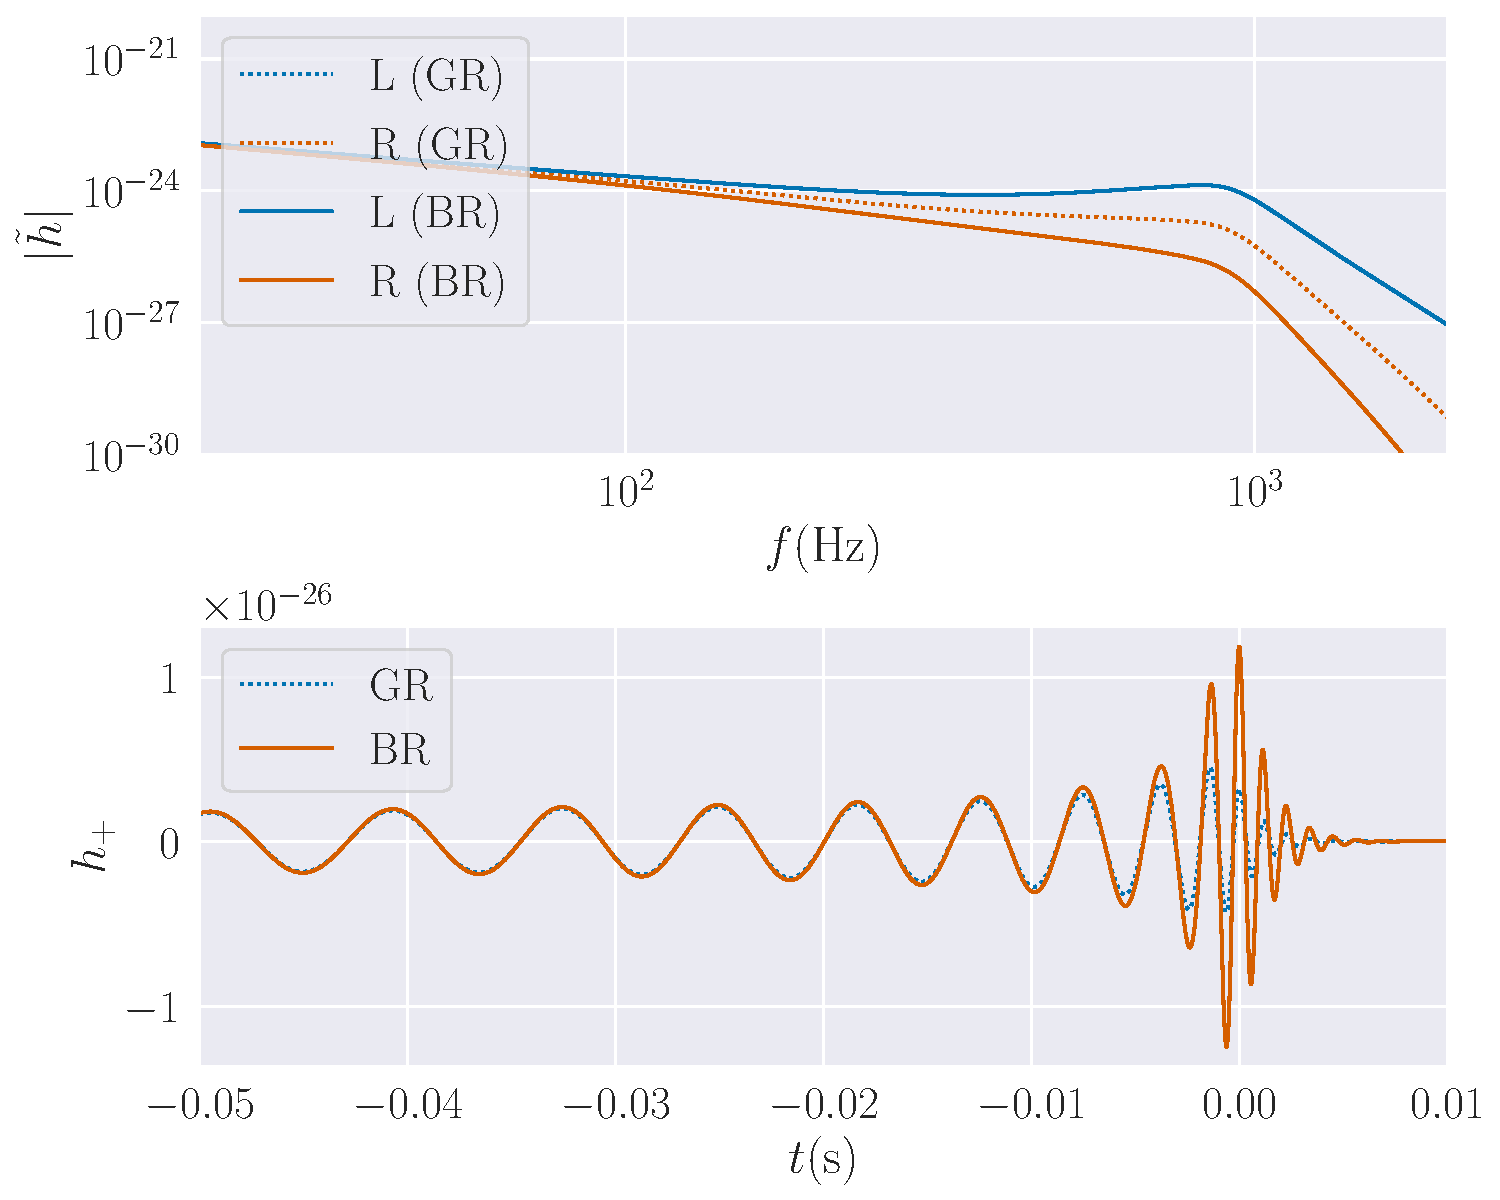
\includegraphics[width=\columnwidth]{figures/birefringence.pdf}
    \caption{
        The observed Fourier amplitude of two polarizations of an simulated GW signal with and without birefringence.
        The amplitudes as GR predicts are shown in dotted lines with blue and orange colors representing the left-handed and right-handed polarizations.
        The amplitudes with birefringence are shown in solid lines with blue and orange colors representing the left-handed and right-handed polarizations.
        This shows the effect of amplitude birefringence with the frequency dependence.
    }
    \label{fig:birefringence}
\end{figure}

% Parameter estimation
The major objective of this study is to constrain GW amplitude birefringence, which is represented by the opacity parameter $\kappa$.
To constrain $\kappa$, we perform PE with data from the third GW transient catalog \citep{GWTC-2.1, GWTC-3}, GWTC-3, using Bilby, a Bayesian toolkit for GW data analysis which is able to calculate posteriors of GW parameters based on interferometer data and priors for the parameters in question \citep{Bilby}. 
We set the prior on $\kappa$ to a uniform distribution between $-1$ and $1$, and perform PE using the modified waveforms.
In both case, we use the same PE configuration as in \citet{GWTC-2.1, GWTC-3} for each individual events.
We also perform test to check if the PE could recover the PE done by LIGO-Virgo-KAGRA Collaboration (LVK) in \citet{GWTC-2.1, GWTC-3}.
We set the prior on $\kappa$ to be a $\delta$ function at $0$, which is the same as using GR.
These control tests result can be found in the data release.

\section{Results}
\label{sec:Results}
\subsection{Result on GWTC-3}
% Stacked kappa posterior plot
\begin{figure}[h]
    \script{kappa_stacked.py}
    \includegraphics[width=\columnwidth]{figures/kappa_stacked.pdf}
    \caption{
        The posterior of $\kappa$ for all 69 events included in this study.
        Each color represent a different event.
        These posterior are used to calculate the population constraint on $\kappa$ in the following.
    }
    \label{fig:kappa_stacked}
\end{figure}

% How to calculate the combined posterior
In figure \ref{fig:kappa_stacked}, we show the individual posterior of $\kappa$ of each events obtained from PE.
We assume $\kappa$ is different for each event, and the population distribution of $\kappa$ is a Gaussian distribution with mean $\mu$ and standard deviation $\sigma$.
We then performed hierarchical modeling to construct the likelihood function of $\mu$ and $\sigma$ given interferometer data.
To sample the posterior distribution of $\mu$ and $\sigma$, we used a generic sampling package, flowMC \citep{flowMC}, with prior of $\mu$ and $\sigma$ being uniform distributions.
The posterior of $\mu$ and $\sigma$ are shown in figure \ref{fig:corner_Gaussian}.

% Corner plot of mean and standard deviation of kappa
\begin{figure}[h]
    \script{corner_Gaussian.py}
    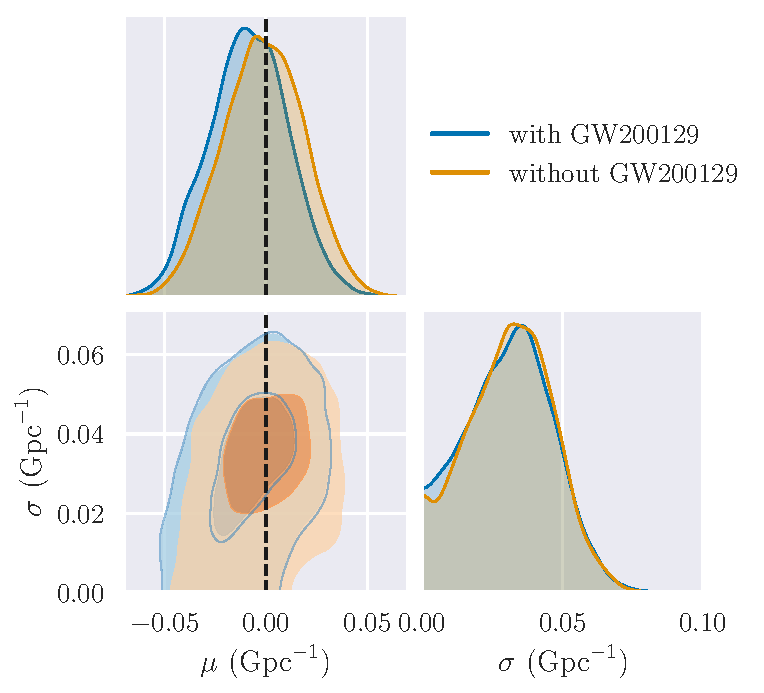
\includegraphics[width=\columnwidth]{figures/corner_Gaussian.pdf}
    \caption{
        The posterior of $\mu$ and $\sigma$ of the population distribution of $\kappa$.
        2D contour plot shows $39.35\%$ and $90\%$ confidence level.
        Orange line represent the median of $\mu$ and $\sigma$, which are \variable{output/mu_median.txt} and \variable{output/sigma_median.txt} respectively,.
        The mean of $\mu$ and $\sigma$ are \variable{output/mu_mean.txt} and \variable{output/sigma_mean.txt}, respectively.
    }
    \label{fig:corner_Gaussian}
\end{figure}

% Constraint on $\kappa$
We then calculate the constraint on $\kappa$ from the posterior of $\mu$ and $\sigma$.
We generated a Gaussian distribution for each sample of $\mu$ and $\sigma$.
The Gaussian distributions were then added up to obtain the population distribution of $\kappa$.
The mean of the population distribution of $\kappa$ is \variable{output/kappa_mean.txt}.
Note that GR is recovered if $\kappa$ is $0$.

% Comparison with previous studies
In \citet{Maria_2021}, the authors gave a constraint on GW amplitude birefringence by performing statistical analysis on GWTC-2.
We convert the constraint to the same format as ours to make comparison.
They were able to constrain $\kappa$ to be $|\kappa| \lesssim 0.74$ at $1 \sigma$.
We were able to obtain a tighter constraint on $\kappa$ with $|\kappa| \lesssim 0.04$ at $1 \sigma$.
This is a order of magnitude improvement in constraining $\kappa$.
This is due to the fact that we have much more events from GWTC-3 compared to GWTC-2.

% Violin plot
In figure \ref{fig:violin_kappa}, we show the posterior of $\kappa$ for each events in the form of violin plot.
There are some events with $\kappa$ distribution deviate from $\kappa=0$.
Also, there are some events with bimodal $\kappa$ distribution.
We are going to discuss some of these events in the following.

\begin{figure*}[ht]
    \script{violin_kappa.py}
    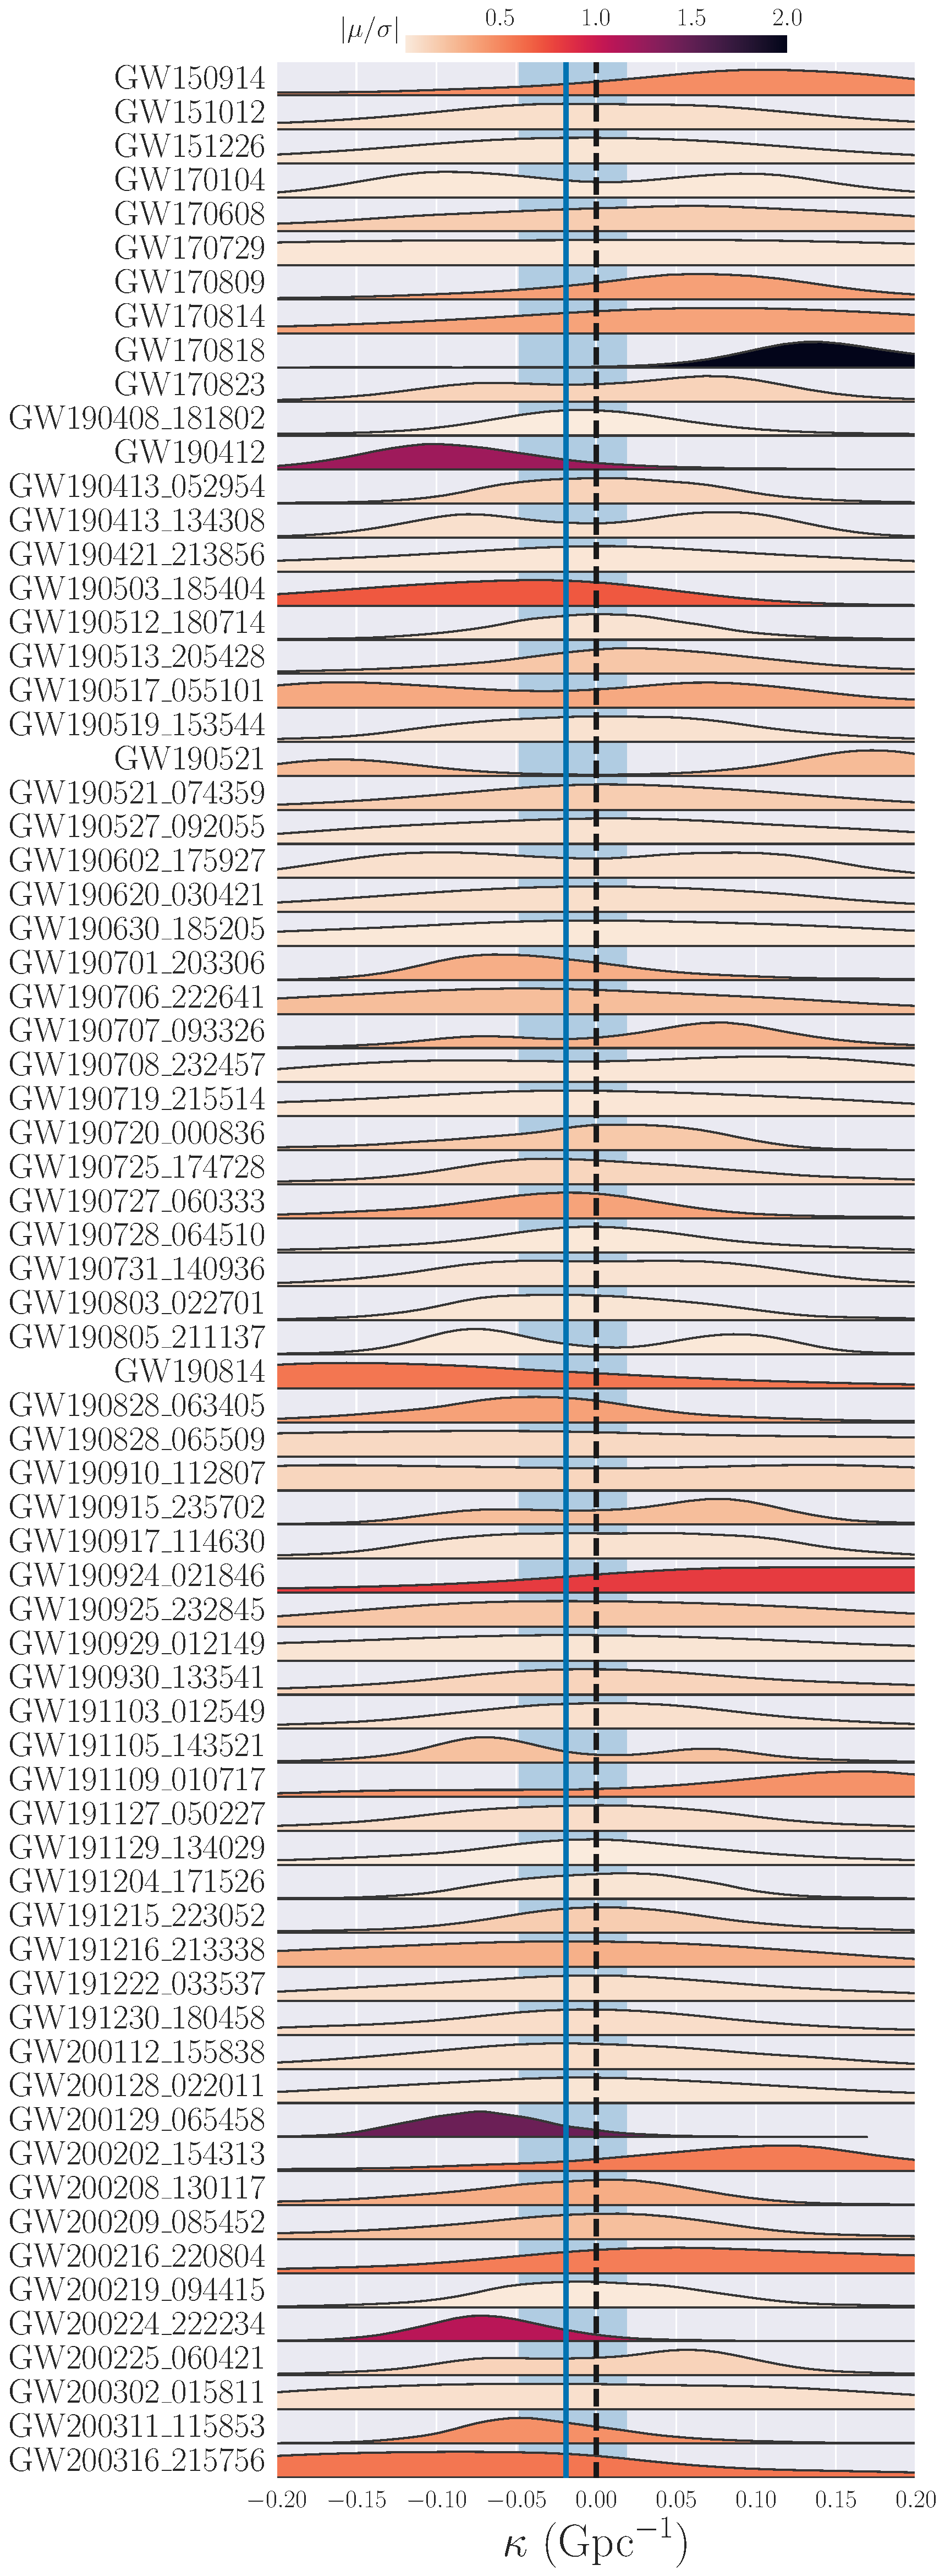
\includegraphics[width=\textwidth]{figures/violin_kappa.pdf}
    \caption{
        The violin plot shows the posterior of $\kappa$ for all 69 events included in this study.
        Each violin represents a different event.
        The violins are sorted by the quotient of median and standard deviation of the posterior.
        Blue horizontal line represent the median value of $\mu$, and blue region represent 1 $\sigma$ confidence level.
        Orange horizontal line represent $\kappa=0$.
        This plot shows that there are some events with $\kappa$ distribution significantly deviate from $0$.
    }
    \label{fig:violin_kappa}
\end{figure*}

% Trend (mass & distance)

% Constraining power

% Case study
% Case: GW170818

% Case: GW150914 (example of broken degeneracy)
\subsection{Result on GW150914}
Some events have bimodal $\kappa$ distribution, but before we show a bimodal event, we should understand the mechanism of a unimodal $\kappa$ distribution.
Consider GW150914, the first GW detected by LIGO.
In figure \ref{fig:corner_GW150914}, we show the posteriors of the parameters of GW150914.
With the frequency independent birefringence model, the posteriors for $\cos\iota$ look different from the posteriors assuming GR.
This is because, for a nonprecessing system, there is a degeneracy between $\kappa$ and $\iota$ if the frequency dependence is not included.
To reconstruct the amplitude ratio from the interferometer data, an $\iota$ representing a more face-off inspiral can pair with a positive $\kappa$, or an $\iota$ representing a more face-on inspiral with a negative $\kappa$.
As a result, many pairs of $\iota$ and $\kappa$ can be plausible with the frequency independence.

On the other hand, with the frequency-dependent birefringence model, the posterior looks similar to the GR posterior.
This is because the degeneracy was broken by the frequency dependence, as the effect of birefringence will be different from the one of changing $\iota$.
In this case, the posteriors can recover the GR distributions for the binary parameters,
and the most probable value of $\kappa$ is close to $0$, which means the birefringence is weak or absent, and GR can be recovered.

\begin{figure}[h]
    \script{corner_GW150914.py}
    \includegraphics[width=\columnwidth]{figures/corner_GW150914.pdf}
    \caption{
        The posterior of $\kappa$, luminosity distance $d_L$ and $\cos{\iota}$ for GW150914.
        Colors in the plot represent the PE with GR done by LVK without cosmological reweighing \citep{GWTC-2.1, GWTC-3}, the PE done by us with both frequency independent and dependent birefringence respectively.
        2D contour plot shows $39.35\%$ and $90\%$ confidence level.
        Note that there is no posterior of $\kappa$ for the PE from LVK, as the LVK PE is based on GR, which does not suggest GW amplitude birefringence.
        This plot shows that frequency independent birefringence create a degeneracy between $\kappa$ and $\iota$, while the frequency dependent birefringence can break it.
    }
    \label{fig:corner_GW150914}
\end{figure}

% Case: GW190521 (massive BBH)
\subsection{Result on GW190521}

Now, we show a bimodal $\kappa$ distribution.
Consider GW190521, the most massive binary black hole merger in the events we included.
The degeneracy between $\kappa$ and $\iota$ cannot be broken by the frequency dependent birefringence model, as shown in figure \ref{fig:corner_GW190521}.
This is because the frequency range of the signal is much smaller due to the large mass of the binary.
The effect of birefringence at different frequency within the range is similar, thus the degeneracy cannot be broken.
This can be a possible reason why the $\kappa$ distribution of GW190521 is bimodal.

\begin{figure}[h]
    \script{corner_GW190521.py}
    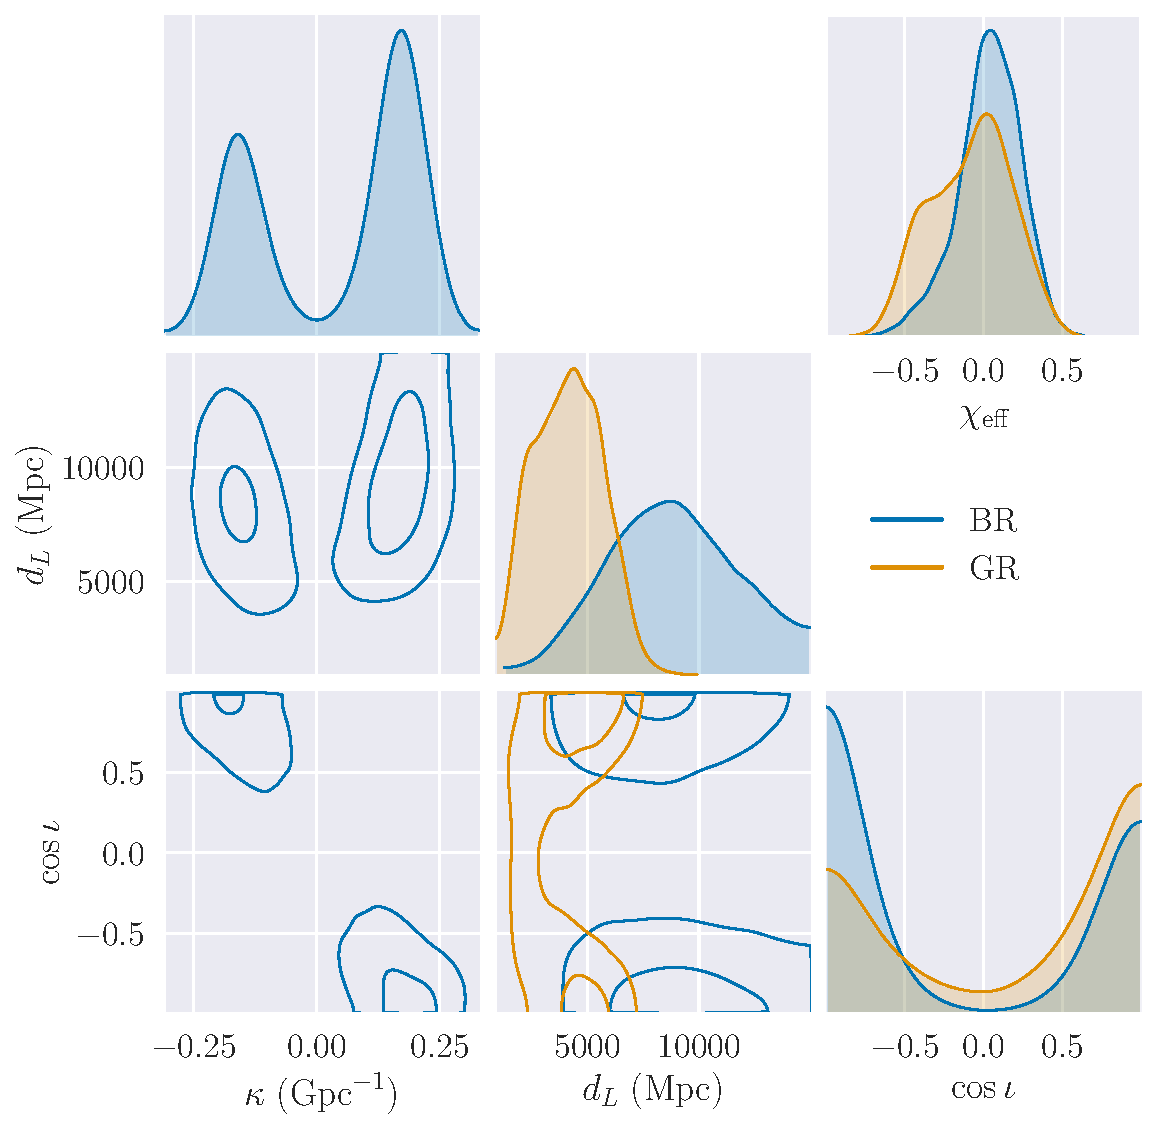
\includegraphics[width=\columnwidth]{figures/corner_GW190521.pdf}
    \caption{
        The posterior of $\kappa$, luminosity distance $d_L$ and $\cos{\iota}$ for GW190521.
        Colors in the plot are the PE with GR done by LVK without cosmological reweighing \citep{GWTC-2.1, GWTC-3} and the PE done by us with the frequency dependent birefringence.
        2D contour plot shows $39.35\%$ and $90\%$ confidence level.
        This plot shows that frequency dependent birefringence cannot break the degeneracy between $\kappa$ and $\iota$.
    }
    \label{fig:corner_GW190521}
\end{figure}

\section{Discussion}
\label{sec:Discussion}

% Reasons for special events
\subsection{Special Events}
% Special event 1: GW190720
For GW190720, we could not perform PE with Bilby successfully.
In LVK PE papers \citep{GWTC-2.1, GWTC-3}, the PE of some events were performed with LALInference \citep{lalsuite} instead of Bilby, GW190720 was one of them.
We successfully migrate LALInference configuration to Bilby for most of these events and recover similar PE results, except for GW190720.
Bilby could not evaluate the likelihood function on Virgo data.
This could bias the population posterior.

% Special event 2: GW200129
For GW200129, past research suggest there could be a potential glitch in Virgo data. \citep{GW200129}
We perform 3 sets of PE to check if the glitch would affect the population posterior of $\kappa$.
In each set, we pick only 2 out of 3 detectors data to perform PE.
The 2 sets of PE results with Virgo data return a $\kappa$ posterior which strongly suggest a negative $\kappa$.
We removed this event from our analysis.
Further investigation is needed to understand the glitch.

% Future work
\subsection{Future Work}
% BNS
A future work is to perform PE on binary neutron star mergers, such as GW170817.
The frequency range of the signal is much larger compared to the binary black hole mergers, thus the difference of the effect of birefringence at different frequency within the range can be more significant.
This can allow us to further constrain the birefringence effect, and the beyond-GR theories that predict it.
However, performing PE on binary neutron star mergers requires much more computational resources.
Therefore, we may need to wait for future PE methods and tools to further our work.

% More observations with higher SNR
Another future work is to apply the same method to more events with higher signal-to-noise ratio (SNR).
LVK will release more events with higher SNR in the future.
Data with higher SNR allows us to obtain more precise PE results, which also allows us to constrain the birefringence effect more precisely.
And more events will allow us to calculate a more constrained population posterior of $\kappa$.

\section{Acknowledgements}
\label{sec:Acknowledgements}
M.~I., K.~W.~K.~W.~ and W.~M.~F.~ are funded by the Center for Computational Astrophysics at the Flatiron Institute, which is supported by the Simons Foundation.
The computational resources used in this work were provided by the Flatiron Institute.

\bibliography{bib}

\end{document}
